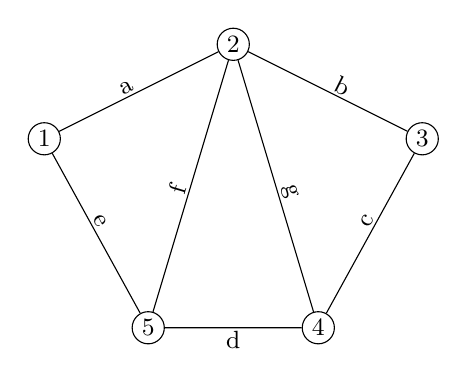
\begin{tikzpicture}[scale=1.2,
        vertex/.style={circle,fill=white,draw=black,inner sep=1.5pt,font=\small},
        elabel/.style={midway,sloped,fill=none,inner sep=1pt,font=\small}
    ]
    %--- vertices ---
    \node[vertex] (v2) at (0,2) {2};
    \node[vertex] (v1) at (-2,1) {1};
    \node[vertex] (v3) at ( 2,1) {3};
    \node[vertex] (v5) at (-0.9,-1) {5};
    \node[vertex] (v4) at ( 0.9,-1) {4};

    %--- edges ---
    \draw (v1)-- node[elabel,above left] {a} (v2);
    \draw (v2)-- node[elabel,above right]{b} (v3);
    \draw (v3)-- node[elabel,above right]      {c} (v4);
    \draw (v5)-- node[elabel,below]      {d} (v4);
    \draw (v1)-- node[elabel,above left]       {e} (v5);
    \draw (v2)-- node[elabel,above left]       {f} (v5);
    \draw (v2)-- node[elabel,above right]      {g} (v4);
\end{tikzpicture}